% !TEX program = xelatex
\documentclass[11pt]{article}
\usepackage[preprint]{coling}
\usepackage{times}
\usepackage{latexsym}
\usepackage[T1]{fontenc}
\usepackage[utf8]{inputenc}
\usepackage{microtype}
\usepackage{graphicx}
\usepackage{booktabs}

\title{ChAAt: A Chinese-specific Ability Atlas for Probing Linguistic Diversity in Large Language Models}
\author{Yankai Wan \\
Jilin University}
\date{}

\begin{document}
\maketitle

\begin{abstract}
We present \textsc{ChAAt}, an auditable system for diagnosing \emph{Chinese-internal linguistic gaps} in large language models. Instead of reporting only aggregate benchmark scores, ChAAt links each capability gap to source-verified items, model outputs, explanations, and item-level statistics. The demonstration combines a 50-item diagnostic core, a 41-item real-exam validity tier, and six open-ended production tasks. On the de-duplicated core, six models are evaluated three times at temperature zero with external search disabled. Overall accuracy ranges from 100\% for DeepSeek Flash and 92\% for GPT-5.4 to 31\% for GPT-4o mini; the latter reaches 28\% on idioms and 13\% on classical Chinese. The interface supports model-by-dimension comparison and drill-down from a low-scoring cell to the exact failed item. ChAAt is designed as a compact diagnostic instrument and reproducible system demonstration, not as a replacement for large-scale Chinese knowledge benchmarks.
\end{abstract}

\section{Introduction}

Popular Chinese LLM benchmarks such as C-Eval \citep{huang-etal-2023-ceval}, CMMLU \citep{li-etal-2024-cmmlu}, and SuperCLUE \citep{xu-etal-2023-superclue} mostly test broad knowledge and reasoning. They rarely isolate the phenomena that make Chinese internally diverse: classical--modern polysemy, idiom misuse, Cantonese aspect markers, honorific direction, and pragmatic ambiguity. A single aggregate score can therefore mask where a model fails and why.

We demonstrate \textsc{ChAAt}, a system that makes this diagnostic process inspectable. Its contributions are: (1) a cross-dimensional interface that connects aggregate rankings to exact failed items and source-grounded explanations; (2) a de-duplicated 50-item diagnostic probe with balanced answer positions and three repeated runs per model; and (3) a multi-rater validation workflow for open-ended answers. We use existing benchmarks as related resources rather than claiming that a compact probe replaces them.

\section{Related Work and Positioning}

\paragraph{Chinese benchmarks.}
C-Eval, CMMLU, and SuperCLUE established broad Chinese evaluation suites. More recent resources focus on specific linguistic dimensions: RegioZH evaluates regional lexical reasoning with 2,607 validated items across five Chinese-speaking regions \citep{zheng-etal-2026-regiozh}; CHENGYU-BENCH contains 2,937 human-verified idiom examples \citep{fu-etal-2025-chengyu}; and YUE-PUB targets Cantonese pragmatic understanding \citep{wu-etal-2026-yue-pub}. These resources show that nominal Chinese proficiency can hide substantial internal variation. ChAAt therefore does not claim maximal coverage. It provides a smaller cross-dimensional probe and an auditable interface for moving from a score to the responsible item.

\paragraph{Evaluation systems.}
EasyJudge demonstrates the value of a user-facing interface for LLM response evaluation \citep{li-sun-2025-easyjudge}. ChAAt differs in scope: it evaluates models on source-verified linguistic tasks, not judge outputs, and exposes per-item evidence alongside model-by-dimension views.

\begin{table*}[t]
\centering
\small
\resizebox{\textwidth}{!}{%
\begin{tabular}{@{}p{2.0cm}p{2.5cm}p{5.2cm}p{5.4cm}@{}}
\toprule
\textbf{Resource / system} & \textbf{Scale} & \textbf{Scope} & \textbf{Primary contribution} \\
\midrule
C-Eval, CMMLU, SuperCLUE & Large & Broad Chinese knowledge and reasoning & Subject-level evaluation and model ranking \\
RegioZH & 2,607 & Regional lexical reasoning & Region-specific coverage and diagnostics \\
CHENGYU-BENCH & 2,937 & Idiom connotation, use, and cloze & Deep coverage of a single lexical phenomenon \\
YUE-PUB & 26,743 & Cantonese pragmatics & Large-scale low-resource pragmatic evaluation \\
EasyJudge & System & Response evaluation & Efficient judge model plus visualization UI \\
\midrule
\textsc{ChAAt} & 50 core + 41 exam + 6 open & Five Chinese-internal dimensions & Score-to-item trace, source-grounded explanation, cross-tier audit \\
\bottomrule
\end{tabular}}
\caption{Positioning against representative Chinese evaluation resources. Scale is not directly comparable because the systems target different scientific questions.}
\label{tab:related}
\end{table*}

\section{System and Benchmark Design}

\textsc{ChAAt} is a Streamlit web application plus a command-line evaluation suite. It provides model presets (DeepSeek, Qwen, GLM, GPT, local Ollama), JSON question banks in which every item carries a source reference, exact-match scoring for single/multiple choice and fill-in-the-blank, a rubric scorer for open-ended tasks, per-dimension radar and model$\times$dimension heatmaps, an interpretable capability-gap list, and a calibration script that reports per-item pass rate ($p$) and discrimination ($D$). A review-first demo mode loads precomputed outputs without API credentials or network access.

\begin{figure*}[t]
\centering
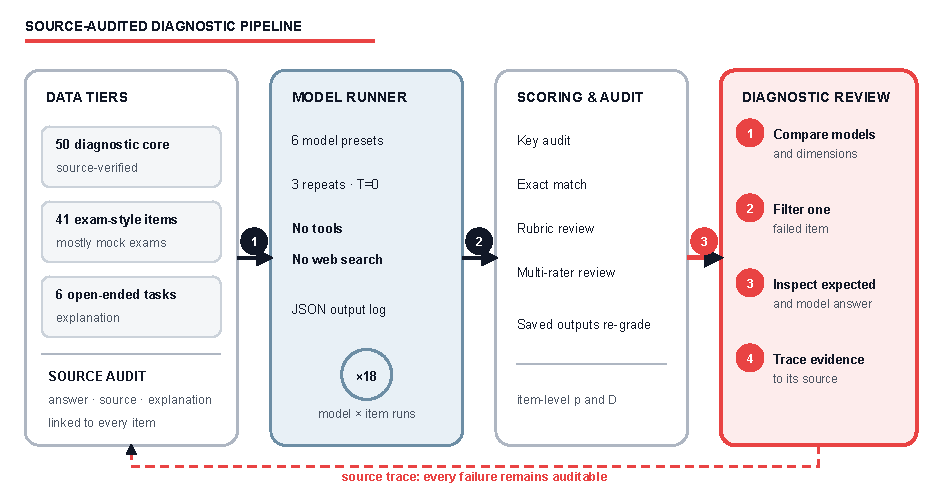
\includegraphics[width=\textwidth]{figs/fig1_architecture.pdf}
\caption{ChAAt system architecture. Source-audited data flow through the evaluation runner, scoring, diagnostics, and review interface without duplicating evidence across components.}
\label{fig:architecture}
\end{figure*}

\begin{figure*}[t]
\centering
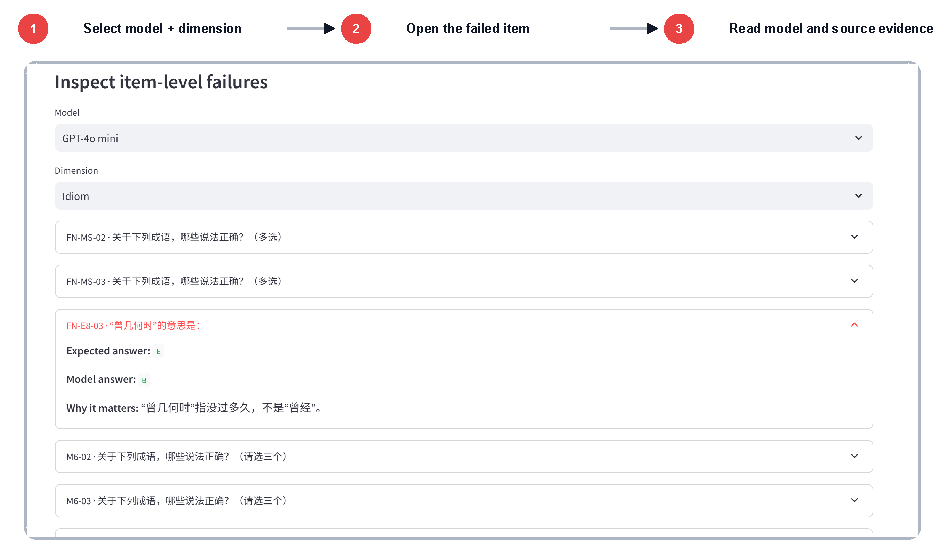
\includegraphics[width=\textwidth]{figs/fig2_interface.pdf}
\caption{The ChAAt item-level failure view. Selecting a model and dimension exposes exact failed items with expected answers, model outputs, and source-grounded explanations while retaining access to the aggregate capability views.}
\label{fig:system}
\end{figure*}

\paragraph{Target users and operation.}
ChAAt targets model evaluators, linguists auditing Chinese-specific coverage, and practitioners choosing models for regional or educational use. A reviewer selects a tier, loads a bundled run or supplies a licensed JSON bank, chooses a model, compares the overall and dimension views, and drills into any failed item. Automatic scoring remains inspectable: changing a key or rubric can re-grade saved outputs without repeating model calls.

\paragraph{Three tiers.}
(1) A de-duplicated \emph{diagnostic core} (50 items, 13 idiom, 15 classical, 9 dialect, 8 slang, and 5 pragmatics) for the main experiment; (2) \emph{real-exam validity} (41 middle/high-school exam items) for ecological grounding; and (3) \emph{open-ended production} (6 tasks) to test explanation rather than option recognition.

\paragraph{Item-writing recipe.} We choose a misconception cluster; write several correct and plausible-but-false statements so that one wrong judgment fails the item; make each distractor correspond to a real error type (modern meaning, literal reading, wrong direction, wrong degree, or wrong aspect); keep options parallel; and verify every statement against an authoritative dictionary or official list (\citealp{zdic} for idioms and classical Chinese, \citealp{wordshk} for Cantonese). This recipe is intended to make failures explainable, not merely difficult.

\begin{table*}[t]
\centering
\small
\resizebox{\textwidth}{!}{%
\begin{tabular}{@{}p{1.7cm}p{5.6cm}p{3.3cm}p{4.3cm}@{}}
\toprule
\textbf{Dimension} & \textbf{Diagnostic item} & \textbf{Expected behavior} & \textbf{Why the trace is useful} \\
\midrule
Idiom & \textit{ceng ji he shi} asks for the conventional rather than literal reading & Time not long ago; not ``a long time ago'' & Connects a failed answer to a dictionary-backed sense \\
Classical & \textit{chu fen shi xiong yi} & Arrange or handle, not punish & Exposes classical--modern sense substitution \\
Dialect & Cantonese \textit{hoi} after a verb & Habitual aspect & Separates lexical recognition from grammatical aspect knowledge \\
\bottomrule
\end{tabular}}
\caption{Representative failure explanations exposed by the same review workflow.}
\label{tab:examples}
\end{table*}

\paragraph{Calibration.} For each item we compute the pass rate $p$ and use the 0.2--0.8 band to prioritize discriminating items; eight all-correct items are retained as coverage anchors. $D$ is the top-half minus bottom-half model accuracy. Final numbers are averaged over three runs at temperature 0.

\section{Experimental Setup}

The six main models are DeepSeek Flash, GPT-5.4, Qwen Max, GLM-4 Plus, GPT-4o mini, and Ollama Qwen3.5-4B. GPT-5.4 mini is evaluated as a matched small-model control; Qwen Plus appeared only in an exploratory validity-tier batch and is not part of the final six-model results. Each main-table model answers 50 items three times at temperature 0. Multi-select items are scored as correct only when the selected letter set exactly matches the key.

\textbf{Statistical reporting.} The unit of analysis is an item ($n=50$). Answer letters were deterministically permuted and balanced separately for the 38 six-option and six four-option multi-select items before the main run, removing answer-position cues. Reported accuracy is the mean over the three runs, with the standard deviation (SD) across runs; because temperature 0 is near-deterministic, most SDs are zero. All 900 main-benchmark responses were non-empty. We report no null-hypothesis significance tests; model comparisons are descriptive. \textbf{Search policy.} No model was given tools or external search access in the main run; DeepSeek's thinking mode was disabled for open-ended answers so that reasoning tokens could not crowd out the response.

\section{Results}

\begin{table*}[t]
\centering
\small
\resizebox{\textwidth}{!}{%
\begin{tabular}{lcccccc}
\toprule
\textbf{Model} & \textbf{Idiom} & \textbf{Classical} & \textbf{Dialect} & \textbf{Slang} & \textbf{Pragmatics} & \textbf{Overall} \\
\midrule
DeepSeek Flash & 100 & 100 & 100 & 100 & 100 & 100 \\
GPT-5.4 & 92 & 87 & 100 & 100 & 80 & 92 \\
GPT-5.4 mini (control) & 92 & 76 & 100 & 100 & 80 & 88.7 \\
Qwen Max & 77 & 78 & 100 & 83 & 73 & 82 \\
GLM-4 Plus & 79 & 67 & 89 & 88 & 67 & 77 \\
Ollama Qwen3.5-4B & 77 & 47 & 56 & 100 & 60 & 66 \\
GPT-4o mini & 28 & 13 & 56 & 50 & 20 & 31.3 \\
\bottomrule
\end{tabular}}
\caption{Accuracy (\%) of the six main models plus the matched GPT-5.4 mini control on the 50-item de-duplicated diagnostic core. Answer positions were deterministically balanced before the main run. The unit of analysis is an item ($n=50$); each cell is the mean of three runs at temperature 0.}
\label{tab:main}
\end{table*}

Table~\ref{tab:main} reports the main results; Figure~\ref{fig:heatmap} and Figure~\ref{fig:radar} omit the matched mini control for visual clarity. The six-model gradient is 100 / 92 / 82 / 77 / 66 / 31. Of the 50 items, 42 show at least one main-model failure and 8 are all-correct coverage anchors. Item-cluster bootstrap intervals (10,000 resamples) are 84--98 for GPT-5.4, 79--96 for GPT-5.4 mini, 71--91 for Qwen Max, 65--88 for GLM-4 Plus, 52--78 for the local 4B model, and 19--44 for GPT-4o mini; DeepSeek Flash is saturated at 100.

\paragraph{Small-model control.} On the de-duplicated core, GPT-5.4 mini reaches 89\% versus 92\% for GPT-5.4. They tie on 43 items; the mini model wins FN-E8-02 and HX-23, while GPT-5.4 wins HX-02, HX-04, HX-06, HX-21, and HX-22. The close result suggests that the aggregate difference is driven by a small set of items rather than a uniform advantage.

For the closest comparison, DeepSeek Flash and GPT-5.4 disagree on four items and have zero discordant preferences in the opposite direction; an exact two-sided McNemar test gives $p{=}0.125$. With 50 items, this difference is not statistically significant, so we report the ranking as descriptive.

\begin{figure}[t]
\centering
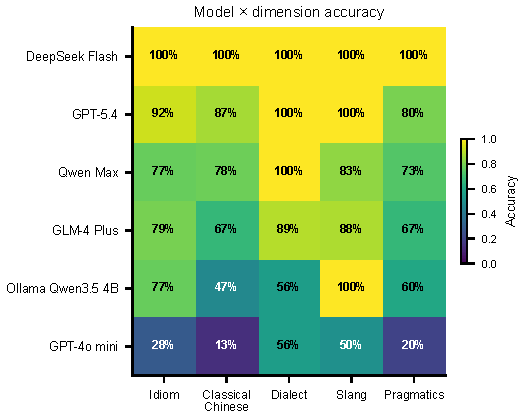
\includegraphics[width=\columnwidth]{figs/fig1_heatmap.pdf}
\caption{Model $\times$ dimension accuracy on the 50-item de-duplicated ChAAt diagnostic core. Each cell is the mean of three runs at temperature 0.}
\label{fig:heatmap}
\end{figure}

\begin{figure}[t]
\centering
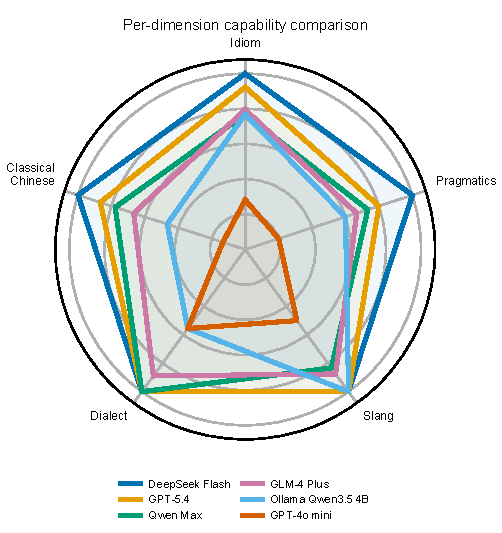
\includegraphics[width=0.9\columnwidth]{figs/fig2_radar.pdf}
\caption{Per-dimension accuracy profile of the six main models on 50 items; each value is the mean of three runs at temperature 0.}
\label{fig:radar}
\end{figure}

\paragraph{Validity tier.} On the 41 real-exam items, DeepSeek Flash and Qwen Max score 100\%, followed by GPT-5.4 at 92.7\%, GLM-4 Plus 85.4\%, Ollama Qwen3.5-4B 80.5\%, and GPT-4o mini 51.2\%. Nine items show broad model splits and 16 additional items show non-uniform performance; 16 are all-correct. Real-exam items therefore provide authority while remaining relatively easy for frontier models.

\paragraph{Production tier.} Two raters independently scored all 36 answers (exact agreement 30/36; within 0.5 points 32/36; ICC(2,k)=0.90; quadratic weighted kappa 0.73), followed by adjudication of six disagreements. A blind third rater then scored all 36 responses. Three-rater reliability was ICC(2,1)=0.888 and ICC(2,k)=0.960, with mean pairwise quadratic weighted kappa 0.740. Two-rater means were 94.6\% for DeepSeek Flash and GPT-5.4, 85.7\% for GLM-4 Plus, 82.1\% for Qwen Max, 78.6\% for the local 4B model, and 57.1\% for GPT-4o mini. The blind third-rater scores were 100.0\% for GPT-5.4; 92.9\% for DeepSeek Flash and Qwen Max; 85.7\% for GLM-4 Plus and the local 4B model; and 57.1\% for GPT-4o mini. With only six tasks, we report both views rather than treating their small ranking differences as a stable model ordering.

\paragraph{Item-level discrimination.} With six models, the highest empirical discrimination is $D{=}0.67$. It occurs on seven items spanning classical polysemy and function words, idiom misconception clusters, Cantonese grammar, and pronunciation. Their overall pass rates range from 17\% to 83\%, so high discrimination is not synonymous with near-zero accuracy. The small number of pragmatics items ($n{=}5$) makes that dimension exploratory rather than population-representative.

\paragraph{Robustness probe.} We rewrote ten discriminating items while preserving their targets and answer semantics, then evaluated each model once. Accuracy on the matched original subset was 100/70/80/83/50/37 for DeepSeek Flash, GPT-5.4, Qwen Max, GLM-4 Plus, the local 4B model, and GPT-4o mini, respectively; on paraphrases it was 100/100/90/80/90/60. The rank correlation is weak and non-significant ($\rho{=}0.47$, $p{=}0.35$, six models). On five additional option-free tasks scored by independent rubric review, accuracy ranged from 80\% for DeepSeek Flash to 55\% for GLM-4 Plus. These probes provide no evidence of a systematic collapse under surface paraphrase, but both are too small to establish contamination resistance or enter the main ranking.

\section{Analysis and Error Taxonomy}

Representative failure patterns are: classical--modern polysemy (weak models read modern senses into classical contexts); dialect aspect markers (some multilingual models confuse the four markers); honorific direction (\textit{linglang}/\textit{quanzi}, \textit{fushang}/\textit{hanshe}); pronunciation (\textit{tian}, \textit{quan}, \textit{gong}); and slang taken literally. These errors form an interpretable capability gap that \textsc{ChAAt} surfaces for each evaluated model.

\section{Limitations}

The 50-item core is a diagnostic probe, not a population-level estimate of Chinese competence. Dimension sizes range from five pragmatics items to fifteen classical items, and the six-model leaderboard should not be generalized to other model families or newer checkpoints. Cantonese items are sourced from words.hk; formal native-speaker validation remains necessary. The 41 real-exam items improve ecological grounding but do not establish construct coverage. All 36 open-ended answers were scored by two independent raters, six disagreements were adjudicated, and all 36 were subsequently scored by a blind third rater. RegioZH, CHENGYU-BENCH, and YUE-PUB are positioned as complementary resources; running the exact same model set on their licensed releases is the next external-validity step.

\section{Demo Plan}

The live demo loads six precomputed model runs without an API key. A reviewer can compare overall and dimension scores, select a model and dimension, and expand an exact failed item to inspect the expected answer, model output, and source-grounded explanation. A short screencast is included with the submission so that the interface can be evaluated without external services.

\section*{Software and Data Availability}

The software is released under the MIT License. ChAAt-authored diagnostic items are released under CC BY 4.0. Third-party exam excerpts are not redistributed in the public package; their sources and derived statistics are documented separately. Dictionary sources (\citealp{zdic}; \citealp{wordshk}) are cited where items were verified. The submission package includes the interface, precomputed demo data, evaluation scripts, and an MP4 demonstration.

\section*{Ethics and Broader Impact}

The study evaluates model outputs and does not collect personal data or involve human-subject interventions. Human raters scored anonymized model responses. The benchmark contains culturally and regionally specific language; we report limitations and avoid treating one variety as the norm.

\section*{Author Contributions, Funding, and Competing Interests}

Yankai Wan designed and implemented the system, constructed the benchmark, ran the experiments, and wrote the paper. This work received no external funding. The author declares no competing interests.

\bibliography{references}

\end{document}
